
%(BEGIN_QUESTION)
% Copyright 2006, Tony R. Kuphaldt, released under the Creative Commons Attribution License (v 1.0)
% This means you may do almost anything with this work of mine, so long as you give me proper credit

Tegn grafen for utgangen  på denne regulatoren med bare p-ledd. Den er stilt inn med følgende verdier:
\begin{itemize}[noitemsep]
	\item proporsjonalbånd 20\%
	\item bias 50 \%
\end{itemize}

%Graph the output of this proportional-only controller, assuming a proportional band value of 20\%, a bias value of 50\%, and a control action that is direct-acting:

$$\includegraphics[width=15.5cm]{i01469x01.eps}$$

\vskip 20pt \vbox{\hrule \hbox{\strut \vrule{} {\bf Suggestions for Socratic discussion} \vrule} \hrule}

\begin{itemize}
\item{} Explain why this trend graph of the PV is unrealistic for a real process, but nevertheless useful for learning how a proportional-only controller is designed to respond to changes in PV.
\item{} How do you suppose the PV would {\it actually} respond in a real process to the conditions shown (or implied) in this trend?  Sketch what you would think would be a more realistic response assuming a properly-tuned proportional-only controller running in automatic mode.
\item{} Identify points on the trend where the PV exhibits a positive rate of change. 
\item{} Identify points on the trend where the PV exhibits a negative rate of change. 
\item{} Identify points on the trend where the PV exhibits zero change. 
\end{itemize}

\underbar{file i01469}
%(END_QUESTION)





%(BEGIN_ANSWER)

$$\includegraphics[width=15.5cm]{i01469x02.eps}$$

%(END_ANSWER)





%(BEGIN_NOTES)

With a proportional band value of 20\%, the gain will be equal to 5.

%INDEX% Control, proportional: graphing controller response

%(END_NOTES)


